\documentclass[cn]{elegantbook}
\usepackage[square,numbers,sort&compress]{natbib}
\newcommand{\upcite}[1]{\textsuperscript{\textsuperscript{\cite{#1}}}}

% title info
\title{模式识别文献综述}
\subtitle{基于深度学习的图像语义分割算法}
% bio info
\author{罗雁天}
\institute{清华大学电子系}
\version{2018310742}
\date{\today}
\logo{logo.png}
\cover{cover.jpg}

\begin{document}

\maketitle
\tableofcontents
\mainmatter
\hypersetup{pageanchor=true}
% add preface chapter here if needed
\chapter*{摘要}
在计算机视觉领域,图像分割指的是将数字图像细分为多个图像子区域(像素的集合)(也被称作超像素) 的过程。图像分割的目的是简化或改变图像的表示形式,使得图像更容易理解和分析。图像分割通常用于定位图像中的物体和边界(线,曲线等)。更精确的,图像分割是对图像中的每个像素加标签的一个过程,这一过程使得具有相同标签的像素具有某种共同视觉特性。

简单来说,图像分割可以看做是像素级别的分类,其在医疗领域、自动驾驶等方面有着重要的应用,在目前的算法研究中,图像分类可以分为语义分割和实例分割。

本文主要从图像语义分割的方向进行调研,介绍了近几年来基于深度学习的图像语义分割算法,并且对这些算法进行对比与总结,最后提出了对图像分割未来方向的展望。

~\\

\noindent\textbf{关键字:图像语义分割;深度学习;全卷积网络;条件随机场}

\chapter*{Abstract}
In the field of computer vision, image segmentation refers to the process of subdividing a digital image into multiple image sub-regions (a collection of pixels) (also referred to as superpixels). The purpose of image segmentation is to simplify or change the representation of the image, making the image easier to understand and analyze. Image segmentation is often used to locate objects and boundaries (lines, curves, etc.) in an image. More precisely, image segmentation is a process of tagging each pixel in an image, which results in pixels with the same tag having some common visual characteristics.

In short, image segmentation can be regarded as a pixel-level classification, which has important applications in the medical field and automatic driving. In the current algorithm research, image classification can be divided into semantic segmentation and instance segmentation.

This paper mainly investigates the direction of image semantic segmentation, introduces the image semantic segmentation algorithm based on deep learning in recent years, and compares and summarizes these algorithms. Finally, it puts forward the prospect of the future direction of image segmentation.

~\\

\noindent\textbf{Key Words: Image Semantic Segmentation; Deep Learning; Fully Convolutional Networks; Conditional Random Field}

\chapter{引言}
图像分割(Segmentation)指的是将数字图像细分为多个图像子区域(像素的集合)(也被称作超像素)的过程。图像分割的目的是简化或改变图像的表示形式,使得图像更容易理解和分析。图像分割通常用于定位图像中的物体和边界(线,曲线等)。更精确的,图像分割是对图像中的每个像素加标签的一个过程,这一过程使得具有相同标签的像素具有某种共同视觉特性。

图像分割又可以分为图像语义分割(Semantic Segmentation)与实例分割(Instance Segmentation)。语义分割是在像素级别上的分类,属于同一类的像素都要被归为一类,因此语义分割是从像素级别来理解图像的。而实例分割不但要进行像素级别的分类,还需在具体的类别基础上区别开不同的实例。比如说图像有多个人甲、乙、丙,那边他们的语义分割结果都是人,而实例分割结果却是不同的对象。

图像分割在实际应用中非常广泛,在医学影像中来用来进行肿瘤和其他病理的定位、组织体积的测量、计算机引导的手术等,在卫星图像中定位物体,用于人脸识别、指纹识别,近几年在自动驾驶领域图像分割也起着至关重要的作用。

\section{评价指标}
在图像分割领域主要有如下4个评价指标:
\begin{itemize}
	\item pixel accuracy (Acc): 像素准确率;
	\item mean pixel accuracy of different categories (mAcc): 类平均像素准确率;
	\item mean Intersection-over-Union of different categories (mIoU): 类平均识别准确度;
	\item frequency-weighted IoU (fwIoU): 频率加权的识别准确度。
\end{itemize}

其中IoU(Intersection-over-Union)表示预测位置与真实位置之间的重叠程度,IoU越高,预测的位置越准确。图\ref{IoU}表示了IoU的几何意义。

\begin{figure}
	\centering
	\begin{minipage}[t]{0.45\textwidth}
		\centering
		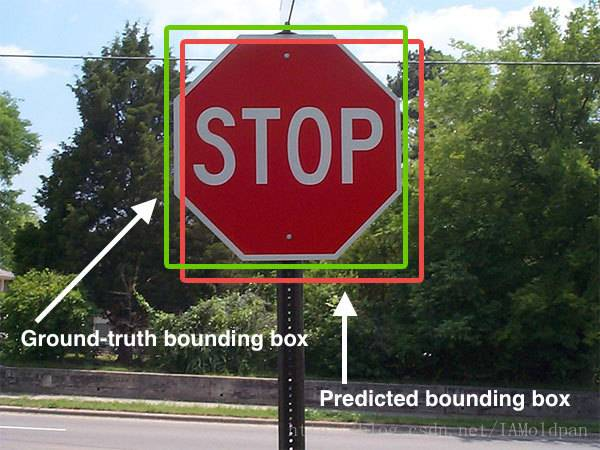
\includegraphics[width=4cm]{images/IoU1.jpg}
	\end{minipage}
	\begin{minipage}[t]{0.45\textwidth}
		\centering
		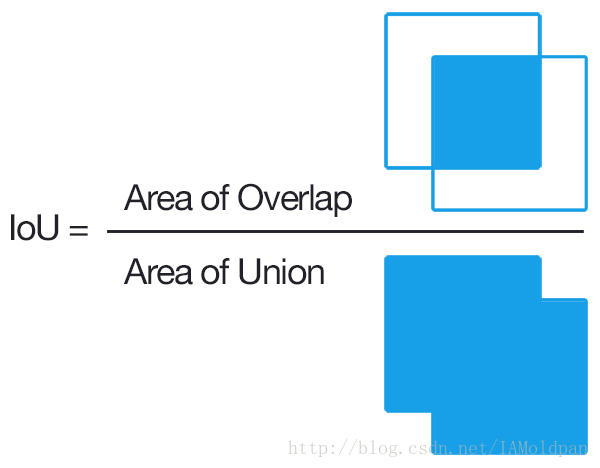
\includegraphics[width=4cm]{images/IoU2.png}
	\end{minipage}
	\caption{\label{IoU}IoU表示含义示意图}
\end{figure}

四个指标的计算方式如式\ref{eval}所示:
\begin{definition}{计算方式}{eval1}
	\begin{equation}
	\label{eval}
	\begin{aligned}
	Acc &= \sum_{i}\frac{n_{ii}}{s} \\
	mAcc &= \frac{1}{n_C}\sum_{i}\frac{n_{ii}}{s_i} \\
	mIoU &= \frac{1}{n_C}\sum_{i}\frac{n_{ii}}{s_i+\sum_{j}n_{ji}-n_{ii}} \\
	fwIoU &= \frac{1}{s}\sum_{i}s_i\frac{n_{ii}}{s_i+\sum_{j}n_{ji}-n_{ii}}
	\end{aligned}
	\end{equation}
\end{definition}

\section{数据集}
图像分割常用的数据集包括PASCAL VOC\upcite{everingham2015pascal}、MS COCO\upcite{2014arXiv1405.0312L}等,包含深度信息图像的数据集有NYUv2\upcite{silberman2012indoor}等。

\begin{itemize}
	\item PASCAL VOC(The PASCAL Visual Object Classification)是目标检测、分类、图像分割领域一个有名的数据集。从2005年到2012年,共举办了8个不同的挑战赛。用于图像分割的VOC2012数据集提供原图以及图像语义分割和图像实例分割两种png图(如图\ref{voc}所示),共分为20类,包括背景为21类,分别如下:
	\begin{itemize}
		\item[-] Person: person;
		\item[-] Animal: bird, cat, cow, dog, horse, sheep;
		\item[-] Vehicle: aeroplane, bicycle, boat, bus, car, motorbike, train;
		\item[-] Indoor: bottle, chair, dining table, potted plant, sofa, tv/monitor.
	\end{itemize}
    \begin{figure}[!h]
    	\centering
    	\begin{minipage}[t]{0.32\textwidth}
    		\centering
    		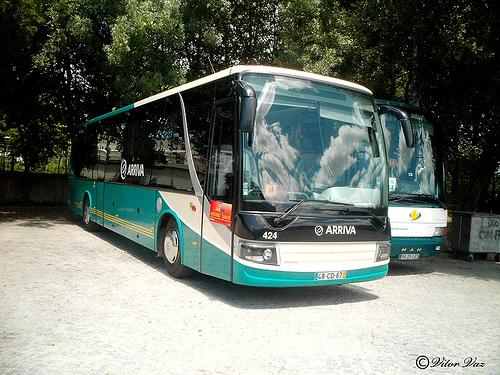
\includegraphics[width=\textwidth]{images/voc1}
    	\end{minipage}
    	\begin{minipage}[t]{0.32\textwidth}
    		\centering
    		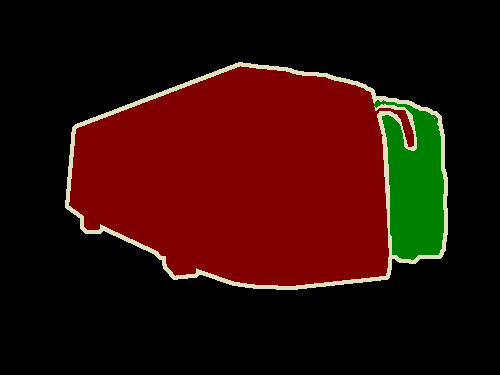
\includegraphics[width=\textwidth]{images/voc1_object.png}
    	\end{minipage}
    	\begin{minipage}[t]{0.32\textwidth}
    		\centering
    		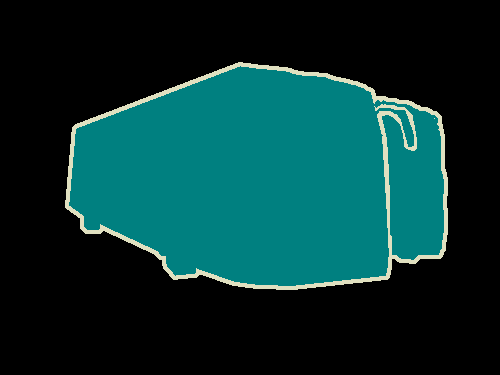
\includegraphics[width=\textwidth]{images/voc1_class.png}
    	\end{minipage}
    	\caption{\label{voc}PASCAL VOC图像分割数据集示例(左图:原始图像;中图:实例分割的标签图;右图:语义分割的标签图)}
    \end{figure}

	\item MS COCO(Common Objects in COntext)是微软建立的数据集。这个数据集也用于多种竞赛:图像标题生成、目标检测、关键点检测和图像分割。图像包括91类目标,328000影像和2500000个label。图\ref{coco}展示了MS COCO举办的各个竞赛中数据集的示例。
	
	\begin{figure}[!h]
		\centering
		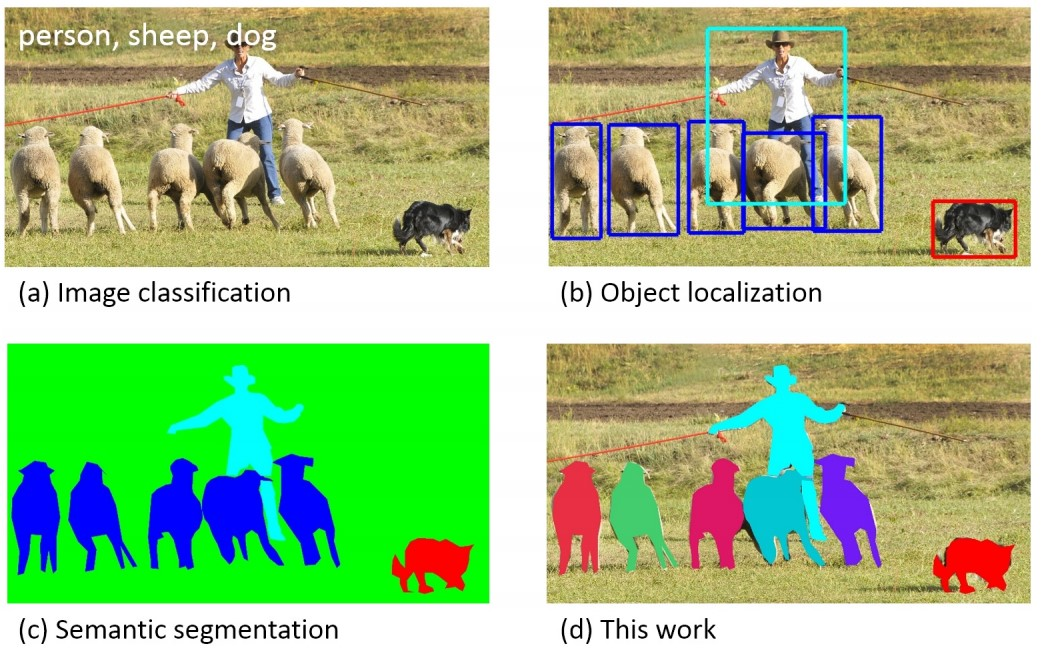
\includegraphics[width=\textwidth]{images/coco}
		\caption{\label{coco}MS COCO数据集多种图像任务示例}
	\end{figure}
	
	\item NYUv2数据集是使用Kinect采集的一系列包含深度信息的图像,包含如下几个部分:
	\begin{itemize}
		\item[-] 有标签的:视频数据的一个子集,伴随着密集多标签。此数据已被预处理以填补缺少的深度标签;
		\item[-] 原始数据集:利用Kinect测得的原始的RGB、Depth、加速度数据;
		\item[-] 工具箱:用于操作数据和标签的有用的工具;
		\item[-] 用于评估的训练和测试部分。
	\end{itemize}
    有标签的数据如图\ref{nyu1}所示。
    \begin{figure}[!h]
    	\centering
    	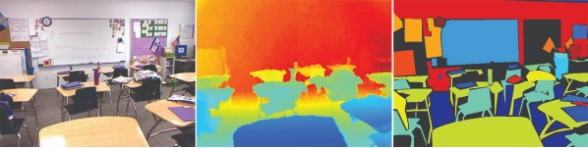
\includegraphics[width=\textwidth]{images/nyu1}
    	\caption{\label{nyu1}NYUv2有标签的数据集示例。(左图:Kinect相机输出的图像;中图:预处理深度信息;右图:添加一系列标签图)}
    \end{figure}
\end{itemize}

\chapter{图像语义分割算法描述}
在深度学习方法流行之前,TextonForest和基于随机森林分类器等语义分割方法是用得比较多的方法。不过在深度卷积网络流行之后,深度学习方法比传统方法提升了很多,所以这里就不详细讲传统方法了。最初的学习方法应用于图像分割就是Patch classification。Patch classification方法,顾名思义,图像是切成块喂给深度模型的,然后对像素进行分类。使用图像块的主要原因是因为全连接层需要固定大小的图像。由于在全卷积网络出现之后对语义分割的效果提升了很多,因此在此也不再详述Patch Classification的方法。

\section{全卷积网络(FCN)}
全卷积网络(Fully convolutional networks, FCN\upcite{long2015fully})于2015年被首次提出,并且获得了当年CVPR的best paper。相比于之前使用带全连接层的卷积神经网络进行图像分割,FCN主要涉及以下三个技术:
\begin{itemize}
	\item 卷积化(Convolutionalization);
	\item 上采样(Upsampling),也叫反卷积(Deconvoltion);
	\item 跳跃结构(Skip Architecture).
\end{itemize}

\subsection{卷积化}
FCN将传统CNN中的全连接层转化为一个个的卷积层。如图\ref{fcn}所示,上图为传统的CNN网络结构(AlexNet\cite{krizhevsky2012imagenet}),前5层是卷积层,第6层和第7层分别是一个长度为4096的全连接层,第8层是一个长度为1000的全连接层。在FCN中,将最后的三层全连接层全都替换为卷积层,卷积核大小分别为(4096,1,1), (4096,1,1), (1000,1,1)。

\begin{figure}[!h]
	\centering
	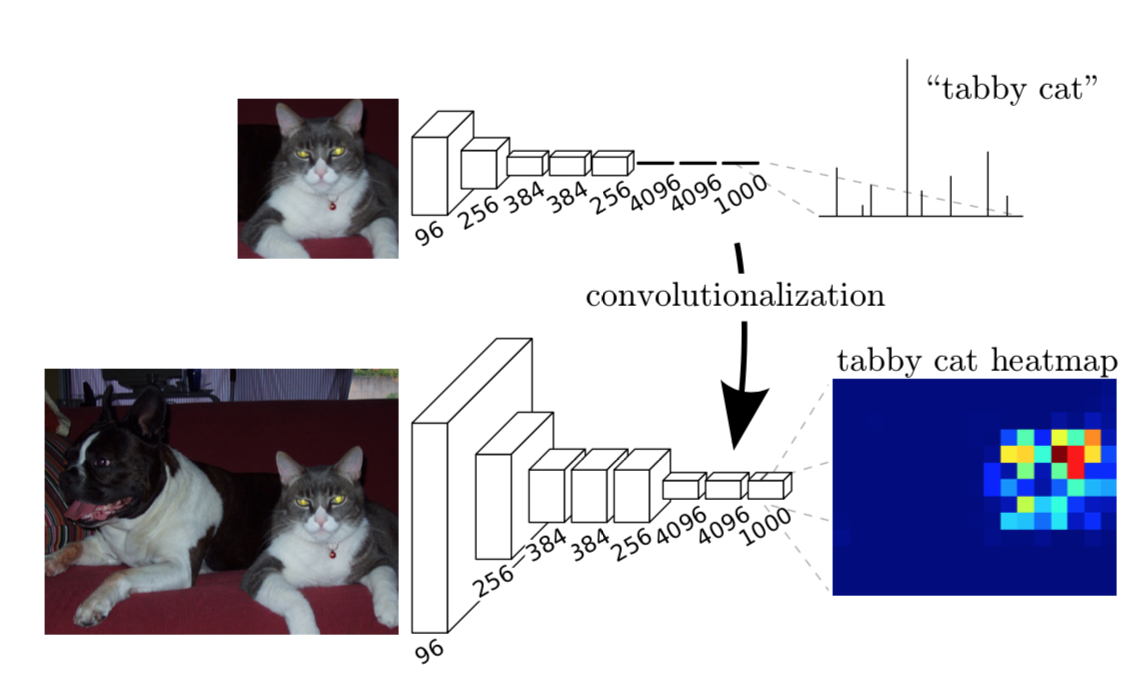
\includegraphics[width=\textwidth]{images/fcn}
	\caption{\label{fcn}FCN与传统CNN对比图}
\end{figure}

网络结构如图\ref{fcn1}所示,虚线上半部分为全卷积网络(蓝:卷积层,绿:max pooling),输入可为任意尺寸的图像,下半部分为反卷积(上采样)结构,最后输出与原图像大小相同,通道数为21(PASCAL VOC数据集20类物体类别+1类背景).

\begin{figure}[!h]
	\centering
	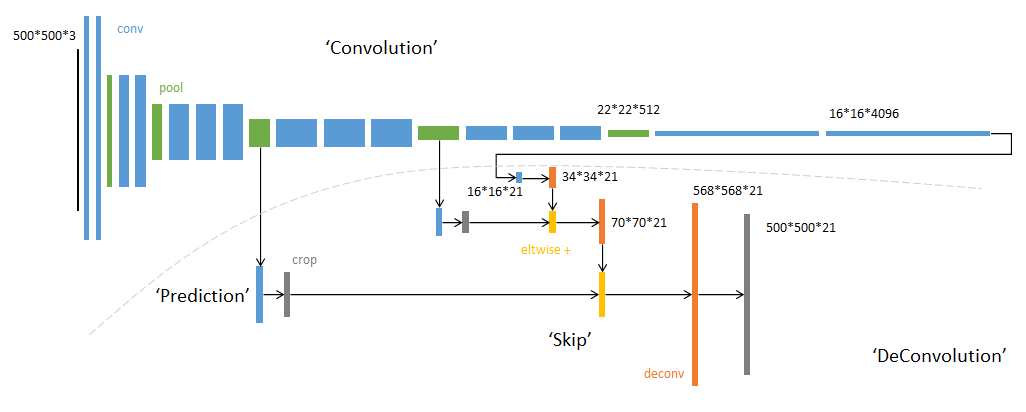
\includegraphics[width=\textwidth]{images/fcn1}
	\caption{\label{fcn1}FCN网络结构示意图}
\end{figure}

\subsection{反卷积}
经过全卷积网络之后得到的feature map相比于原图像要小,为了得到和原图像一样的feature map以便进行像素级的分类,FCN采用反卷积的方式将最后一层的feature map进行放大(图\ref{fcn1}中虚线以下橙色的部分)。

图\ref{deconv}展示了正常卷积与反卷积的对比图,左图展示的正常的no padding no strides情况下的卷积操作,可以看出,卷积之后feature map会变小,右图展示的是no padding no strides情况下的反卷积操作,可以看出反卷积之后feature map会增大。简单来看,反卷积其实可以看做先对feature map进行上采样增加像素,然后再进行卷积的过程,卷积的参数值通过训练得到。

\href{https://github.com/vdumoulin/conv_arithmetic}{https://github.com/vdumoulin/conv\_arithmetic}给出了各种类型卷积的动态图(正常卷积、反卷积以及之后要涉及的空洞卷积),可以通过动态图进一步认识各种卷积操作。论文\cite{dumoulin2016guide}给出了详细的数学公式以及卷积前后feature map大小的变化公式,可以更深一步的认识卷积。


\begin{figure}
	\centering
	\begin{minipage}[t]{0.45\textwidth}
		\centering
		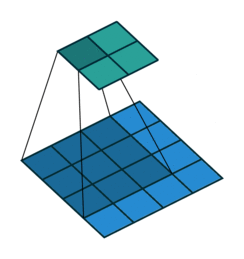
\includegraphics[width=\textwidth]{images/no_padding_no_strides-0.png}
	\end{minipage}
	\begin{minipage}[t]{0.45\textwidth}
		\centering
		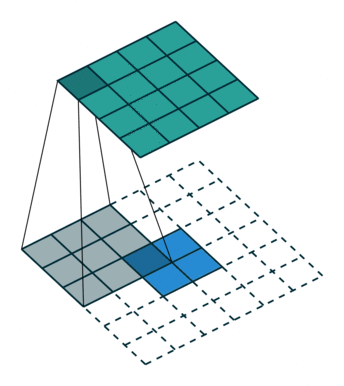
\includegraphics[width=\textwidth]{images/no_padding_no_strides_transposed-0.png}
	\end{minipage}
	\caption{\label{deconv}正常卷积与反卷积对比图}
\end{figure}

\subsection{跳跃结构}
如图\ref{skip}所示展示了FCN中跳跃结构示意图。从图中可以看出,对原图进行卷积conv1、pool1后图像缩小为1/2;对图像进行第二次卷积conv2、pool2后图像缩小为1/4;对图像进行第三次卷积conv3、pool3后图像缩小为1/8,此时保留pool3的featuremap;对图像进行第四次卷积conv4、pool4后图像缩小为1/16,此时保留pool4的featuremap;对图像进行第五次卷积conv5、pool5后图像缩小为1/32,然后把原来CNN操作过程中的全连接编程卷积操作的conv6、conv7,图像的featuremap的大小依然为原图的1/32,此时图像不再叫featuremap而是叫heatmap。其实直接使用前两种结构就已经可以得到结果了,这个上采样是通过反卷积(deconvolution)实现的,对第五层的输出(32倍放大)反卷积到原图大小。但是得到的结果还上不不够精确,一些细节无法恢复。于是将第四层的输出和第三层的输出也依次反卷积,分别需要16倍和8倍上采样,结果过也更精细一些了。这种做法的好处是兼顾了local和global信息。

\begin{figure}[ht]
	\centering
	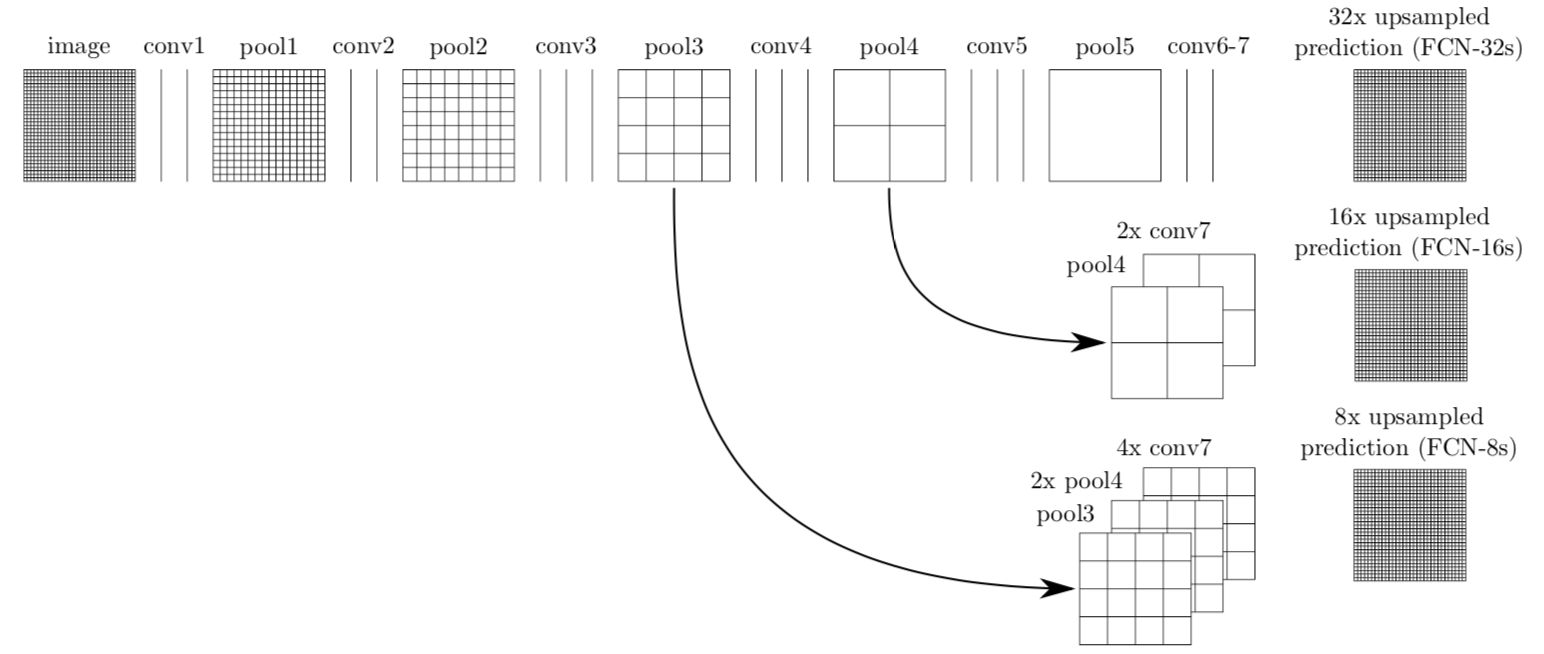
\includegraphics[width=\textwidth]{images/skip.png}
	\caption{\label{skip}跳跃结构示意图}
\end{figure}

\subsection{实验结果}
在此篇论文中,作者分别使用了一次反卷积、两次反卷积以及三次反卷积操作进行实验,并且使用修改过的VGG网络结构进行训练,最后在PASCAL VOC数据集上的性能指标如图\ref{fcnres}所示。由结果图中可以直观的看出,FCN的图像分割结果和ground truth相比已经有了较好的效果,但是边缘部分差距还是较大,在之后的几种算法中会有进一步的提升。

\begin{figure}[!h]
	\centering
	\begin{minipage}[t]{0.85\textwidth}
		\centering
		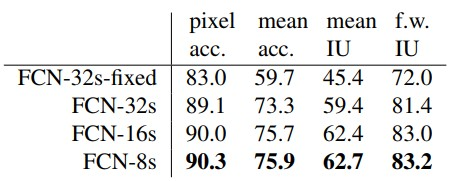
\includegraphics[width=\textwidth]{images/fcnres}
	\end{minipage}
	\begin{minipage}[t]{0.85\textwidth}
		\centering
		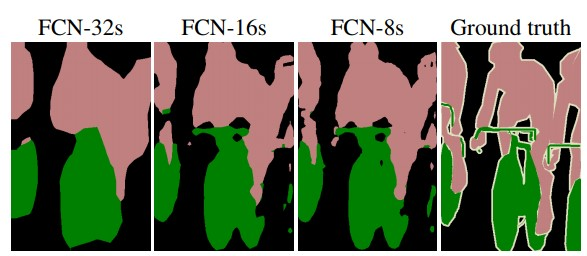
\includegraphics[width=\textwidth]{images/fcnres1}
	\end{minipage}
	\caption{\label{fcnres}实验结果性能指标与PASCAL VOC数据集上的实验效果图}
\end{figure}

\section{DeepLab}
从FCN的实验结果图中可以看出来,虽然分割的整体区域比较正确了,但是分割效果还是比较粗糙,细节不明显。DeepLab v1(文章\cite{chen2014semantic})使用Hole算法(Atrous Algorithm)和条件随机场(CRF)来进一步的提升分割效果,其算法结构图如图\ref{deeplabv1}所示。DeepLab v1收录于ICLR 2015,是DeepLab系列的第一篇文章,之后我们还会介绍该系列的后续文章。

\begin{figure}[!h]
	\centering
	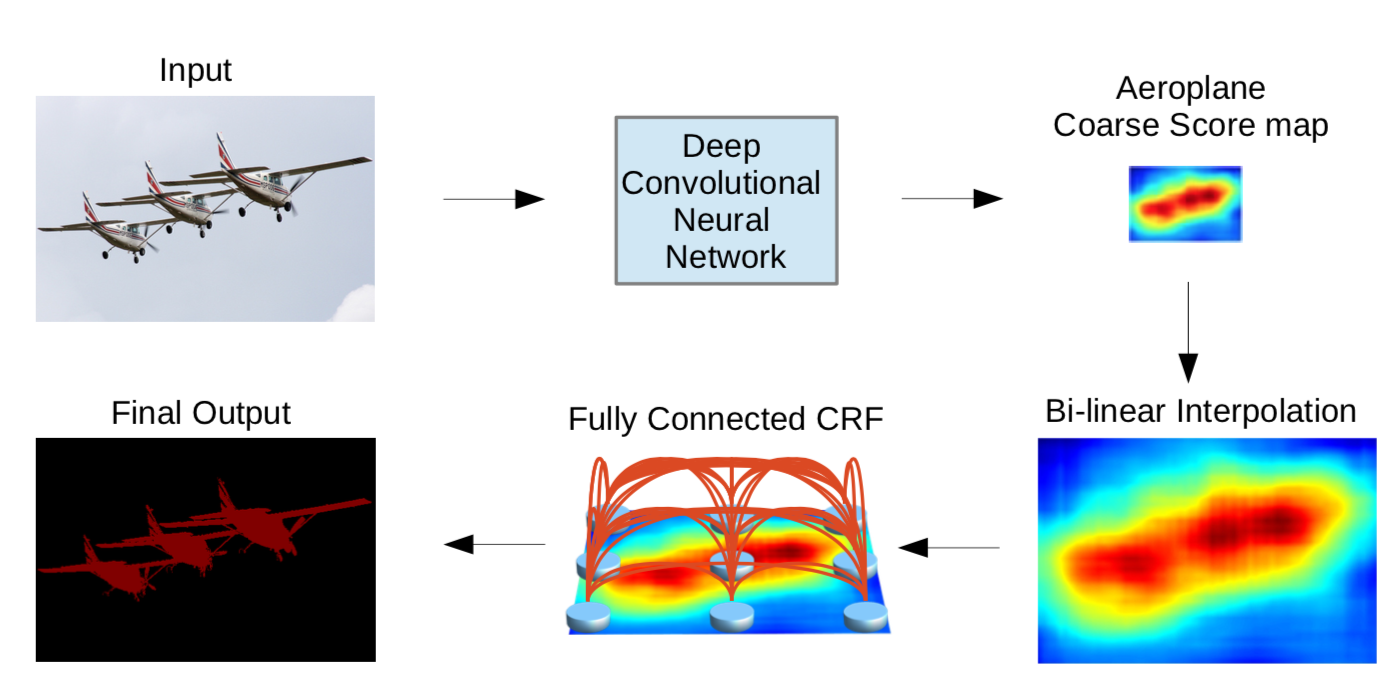
\includegraphics[width=\textwidth]{images/deeplabv1}
	\caption{\label{deeplabv1}DeepLab算法结构示意图}
\end{figure}

\subsection{Hole算法}
由于普通的卷积感受野较小,需要增加池化层来增加感受野,但是池化层又会损失信息,所以使用空洞卷积在不损失信息的情况下增加感受野的范围。

Hole算法又可以看做带孔(Hole)卷积,传统的卷积或者pooling中,一个filter中相邻的权重作用在feature map上的位置都是物理上连续的。而在Hole算法中,一个filter中相邻的权重不一定作用在feature map上的位置都是物理上连续的,而是跟hole size相关的。如图\ref{hole}所示表示的是卷积核大小kernel\_size=3,输入步长input\_stride(也就是hole size)=2,输出步长output\_stride=1的一维带孔卷积示意图。可以看出卷积核作用在输入feature map上的位置不是连续的。后续章节会有关于Hole算法的更详细的介绍,在此不再赘述。


\begin{figure}[!h]
	\centering
	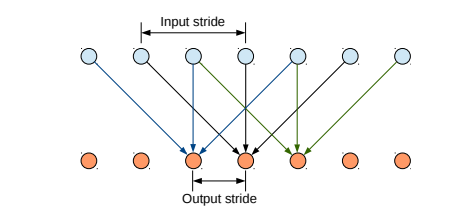
\includegraphics[width=\textwidth]{images/hole}
	\caption{\label{hole}Hole算法示意图}
\end{figure}

\subsection{条件随机场}
只使用全卷积网络能够预测到目标的大概位置但是位置比较模糊,论文\cite{krahenbuhl2011efficient}中提出的全连接条件随机场尝试找到图像像素之间的关系:相近且相似的像素大概率为同一标签,考虑像素的概率分配标签,通过迭代来细化分割的结果。

条件随机场服从吉布斯分布,如式(\ref{gibbs})所示,其中$E(X)$是$x$取某个值的能量,$Z(I)$是归一化的函数。
\begin{equation}
\label{gibbs}
P(X|I)=\frac{1}{Z(I)}\exp(-E(X|I))
\end{equation}

为了做图像分割,只需要后验概率最大,因此只需能量函数最小即可,因此条件随机场优化的目标函数便是能量函数$E(X)$(式(\ref{energy})).
\begin{equation}
\label{energy}
E(x)=\sum_i \psi_i(x_i)+\sum_{i,j} \psi_{i,j}(x_i,x_j)
\end{equation}

能量方程的第一项$\psi_i(x_i)$(式(\ref{unary}))称为一元势函数,用于衡量当像素点$i$的颜色值为$y_i$时,该像素点属于类别标签$x_i$的概率。在DeepLab中,此概率是通过CNN的输出得到的。
\begin{equation}
\label{unary}
\psi_i(x_i)=-\log(P(x_i))
\end{equation}

能量方程的第二项$\psi_{i,j}(x_i,x_j)$称之为成对势函数(pairwise),用于衡量两事件同时发生的概率$p(x_i,x_j)$,我们希望两个相邻的像素点,如果颜色值$y_i,y_j$非常接近,那么这两个像素点$x_i,x_j$属于同一个类别的概率应该比较大才对;反之如果颜色差异比较大,那么我们分割的结果从这两个像素点裂开的概率应该比较大才对。这一能量项正是为了让我们的分割结果尽量从图像边缘的地方裂开,也就是为了弥补之前FCN边缘的地方分割的不足,我们可以采用式(\ref{pairwise})来计算。
\begin{equation}
\label{pairwise}
\psi_{i,j}(x_i,x_j)=u(x_i,x_j)\sum_{m=1}^{M}w^mK_G^m(f_i,f_j)
\end{equation}
其中$K_G$是一个高斯核,用于度量像素点$i$和$j$的特征向量相似度的一个高斯权重项。特征向量$f_i$我们可以用$(x,y,R,G,B)$表示,也就是以像素点的像素值和坐标位置作为特征向量。然后$u(x_i,x_j)$表示两个标签之间的一个兼容性度量。通过最小化式(\ref{energy})的能量函数,我们就可以实现CRF隐变量$X$的推理。

图\ref{crf1}显示了DeepLab中使用CRF迭代来细化分割结果的示意图,从图中可以看出,使用CRF迭代可以使得分割的边缘效果逐渐增强。
\begin{figure}[!h]
	\centering
	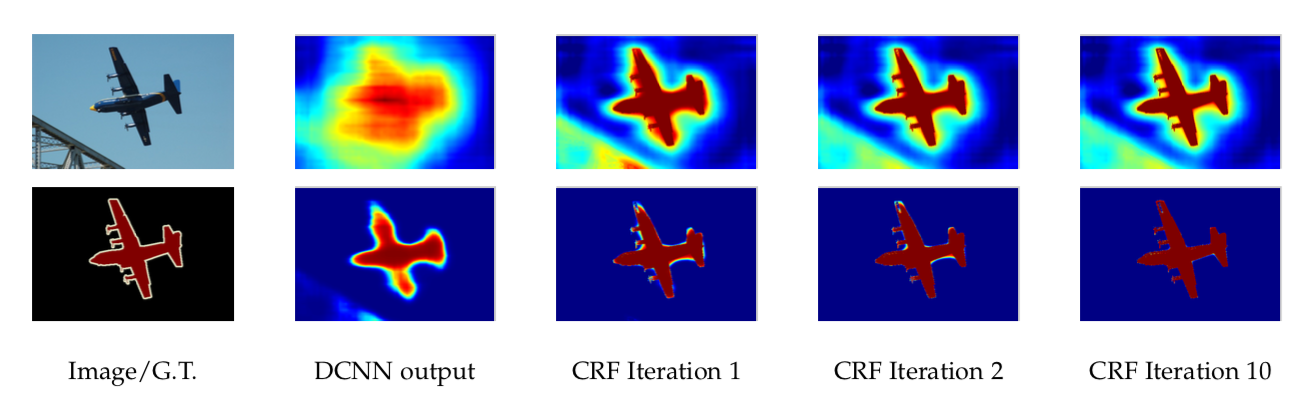
\includegraphics[width=\textwidth]{images/crf}
	\caption{\label{crf1}使用CRF细化分割效果。可以看出,随着迭代次数的增加,图像分割的效果逐渐增强}
\end{figure}

\subsection{网络结构}

\section{DilatedConv}

\section{DeepLab v2}

\section{PSPNet}

\section{DeepLab v3}
\chapter{方法结果对比}

\chapter{总结}



\bibliographystyle{unsrt}
\bibliography{cite}

\end{document}